\chapter{Evaluation}\label{chapter:evaluation}
In diesem Kapitel werden die Ergebnisse der Arbeit evaluiert. Dabei wird zum einen auf den entwickelten Prototypen eingegangen und zum anderen das Konzept und die Anwendung von Augmented Reality im Bildungsbereich evaluiert.

\section{Evaluation des Prototyps}
Dieses Kapitel dient dazu den Prototypen anhand der in Kapitel \ref{chapter:anforderungsanalyse} gestellten Anforderungen zu evaluieren. Dazu wird zunächst das Testverfahren, das parallel zu der Implementierung genutzt wurde beschrieben und im Anschluss der finale Prototyp evaluiert.

\subsection{Tests}\label{sec:Tests}
Während der Entwicklung wurde mit Hilfe von ausführlichen Tests die Funktionalität neuer Features sichergestellt und eine ausführliche Testdokumentation angefertigt. Dadurch sollten Fehler, Probleme und mögliche Verbesserungen entdeckt und festgehalten werden. \\
Das Ziel war es für jedes neue Feature einen Test durchzuführen.\\
Dafür wurde die Anwendung mit Hilfe von Android Studio auf ein Androidgerät geladen und dort getestet.
Dieses bot die Möglichkeit die Tests in einer realistischen, praxisnahen Umgebung durchzuführen, um noch bessere Erkenntnisse über die Alltagstauglichkeit der neuen Features zu erhalten. \\
Als Testgerät diente dabei ein Huawei P30 Pro
Dabei wurden die einzelnen Grundfunktionalitäten auf verschiedenen getestet.

\subsubsection{Augmented Reality}\label{sec:Testdurchführung}
Bei dem Testen neuer AR-Funktionalitäten wurde darauf Wert gelegt, dass die einzelnen Durchläufe in der selben Testumgebung und unter den gleichen Umständen stattfinden, um eine Vergleichbarkeit zwischen den verschiedenen Versionen herzustellen.
So konnte nach jedem Test zusätzlich festgestellt werden, ob sich eventuell die bestehende Eigenschaften im Vergleich zur Vorgängerversion verschlechtert oder verbessert hatten. \\
Zu diesem Zweck wurde für jeden Durchlauf der in Abbildung \ref{fig:Testaufbau} gezeigte Versuchsaufbau gewählt.

\begin{figure}[h!]
\centering
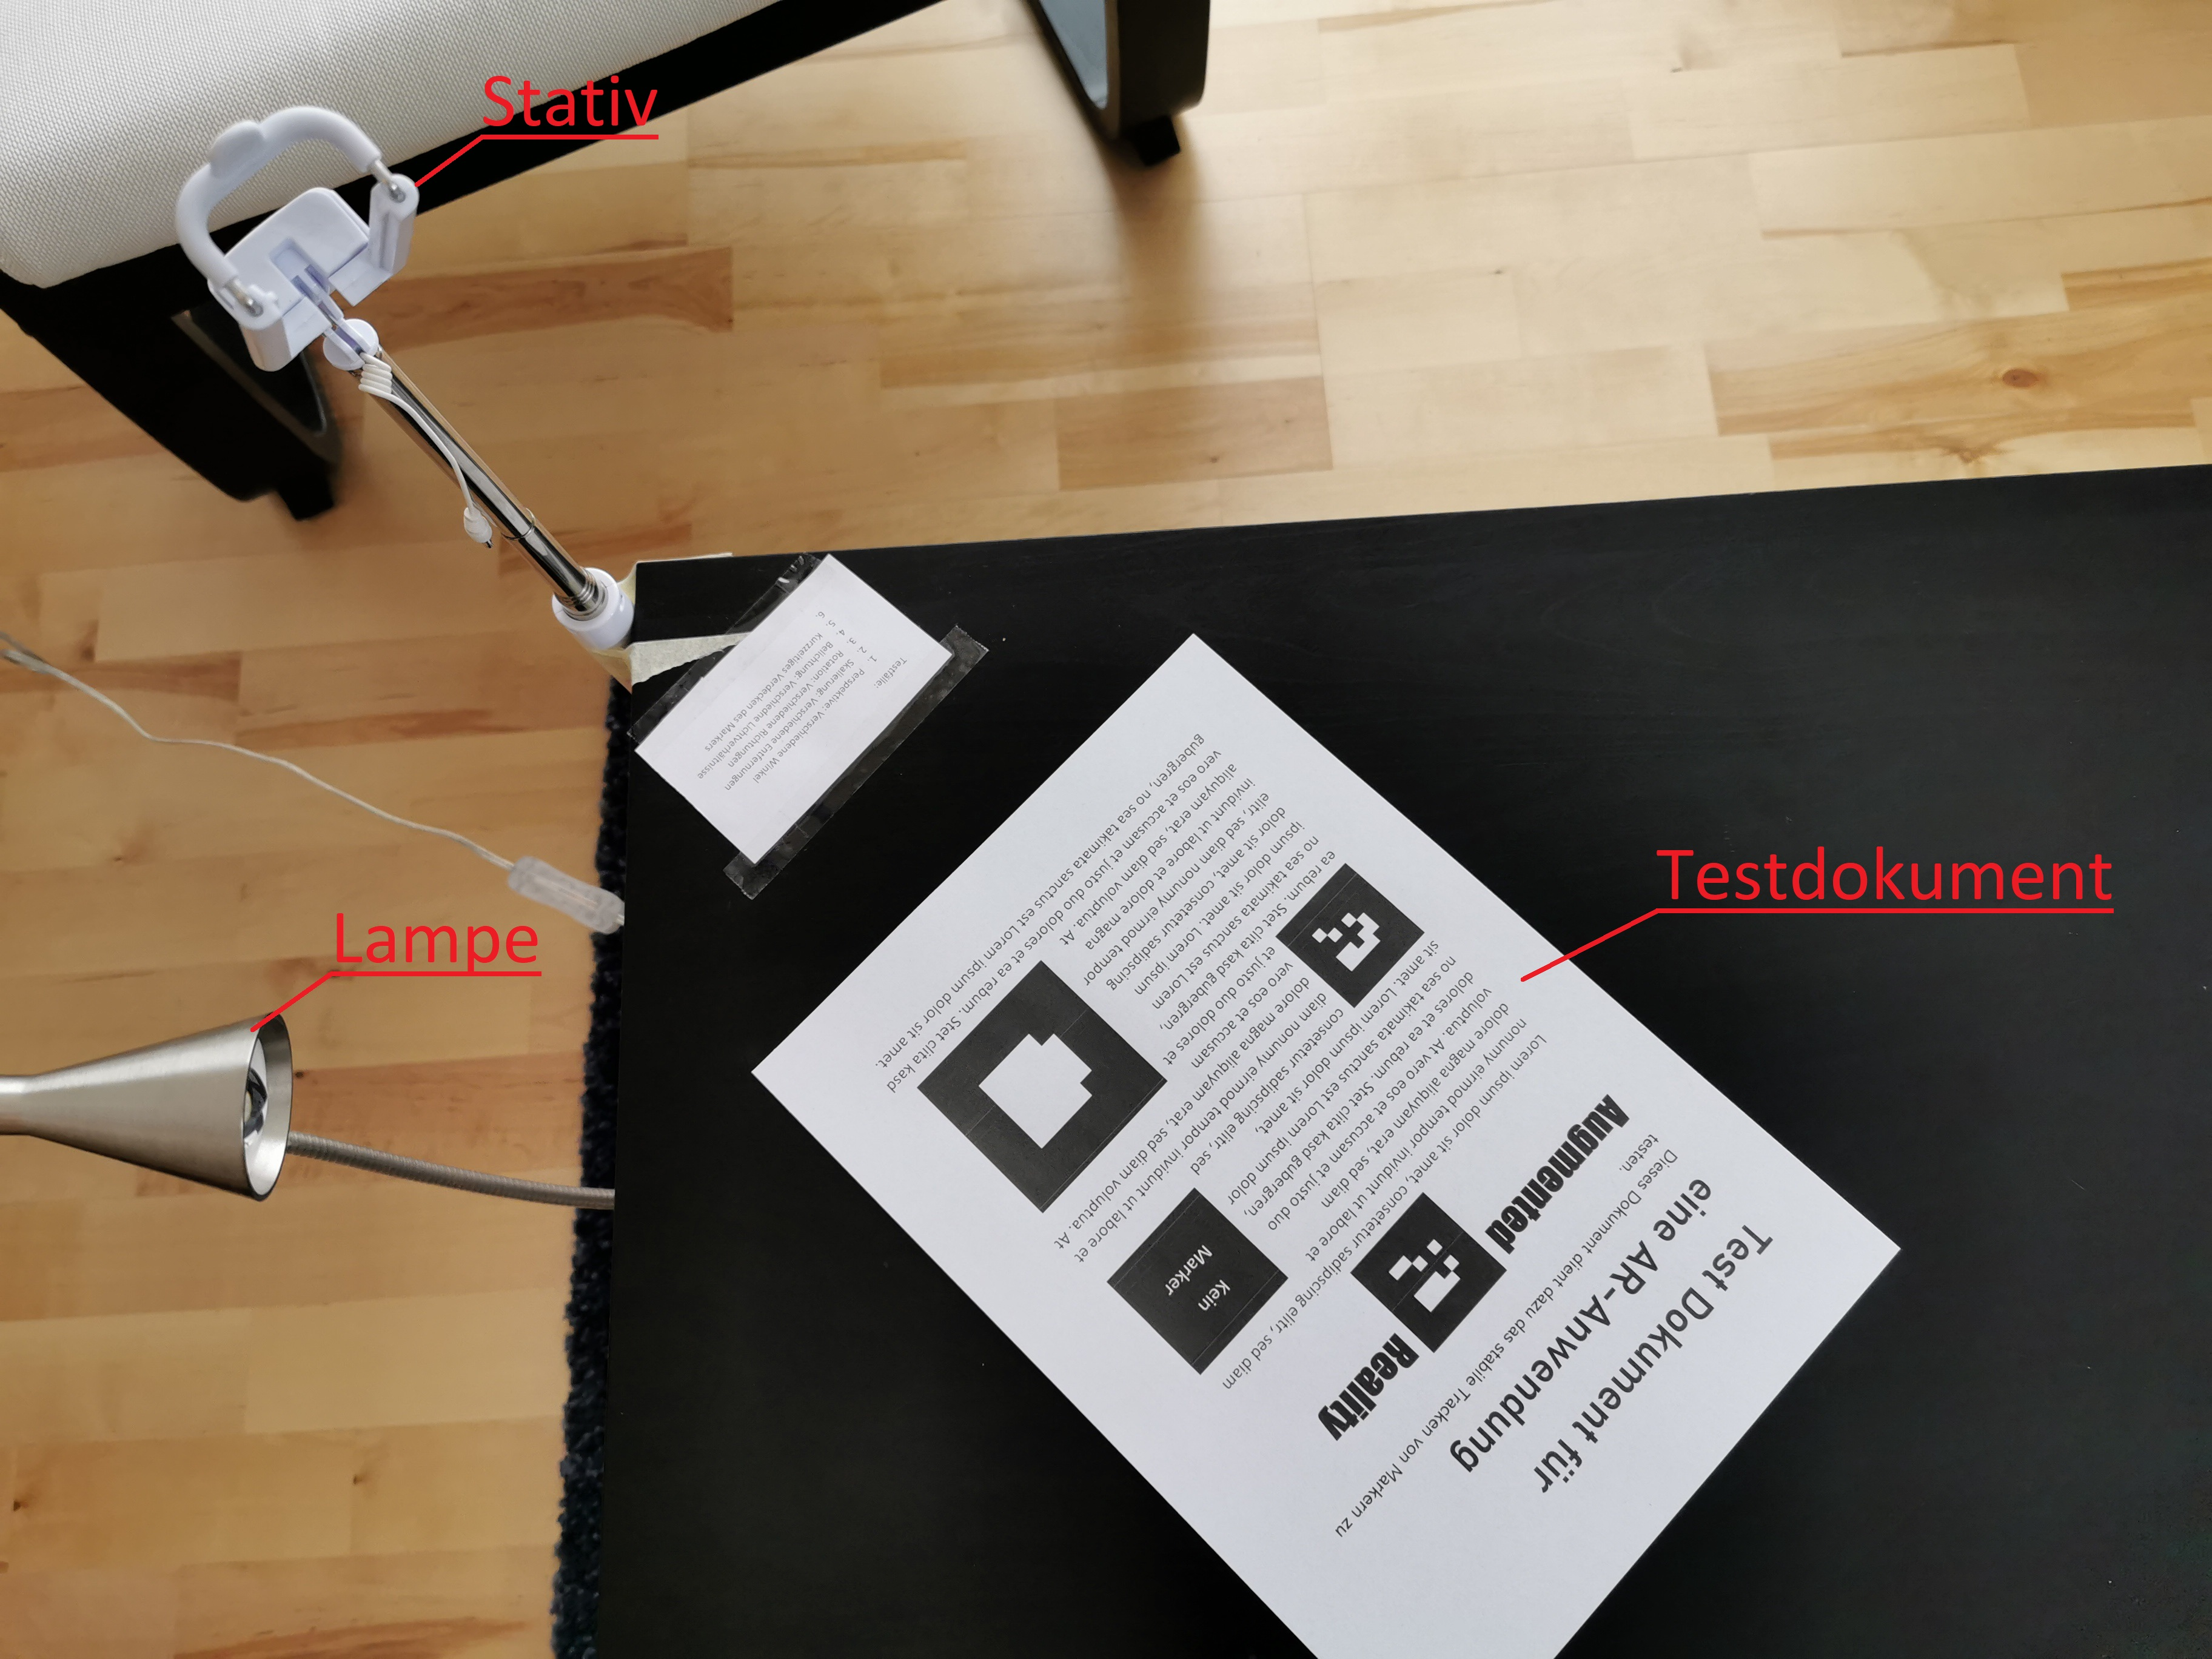
\includegraphics[width=0.7\textwidth]{Abbildungen/Testaufbau.jpeg}
\caption[Testaufbau]{Der Testaufbau für jeden Durchlauf. (Quelle: Eigene Darstellung)}
\label{fig:Testaufbau}
\end{figure}
Zum Testen des Trackings wurde ein Testdokument \todo{Verweis auf Testdokument(Anhang)} angefertigt. Dieses Dokument wurde im Laufe der Entwicklung an die neuen Features angepasst und optimiert. Grundlegend bildet das Dokument einen oder mehrere Marker ab. Gegebenenfalls sind die Marker in Textpassagen eingebunden, um den Schwierigkeitsgrad für die Markererkennung zu erhöhen.\\
Während des Testlaufs wurden jedes mal vier Testfälle durchlaufen, die in Abschnitt \ref{sec:Testfälle} beschrieben werden. Dabei wurden sowohl die Neuerungen getestet, als auch Veränderungen in den bereits bestehenden Features festgehalten.\\
Jeder Testfall wurde dabei mit Hilfe der in Android enthaltenen Funktion \glqq Bildschirmrekorder\grqq aufgezeichnet und in dem entsprechenden Testbericht dokumentiert.\\
Die Testfälle an sich beruhen auf den Eigenschaften des SIFT-Algorithmus, welcher Bildmerkmale extrahiert, die invariant gegenüber Rotation, Translation, Skalierung und partiell invariant gegenüber Helligkeitsveränderungen sind \citep[S. 345]{nischwitz:bildverarbeitung}. Mithilfe des Algorithmus können dieselben Objekte in zwei verschiedenen Aufnahmen wiedererkannt werden.\\
Da auch beim Marker Tracking ein ähnliches Verfahren angewandt werden muss, sind auch hierbei die genannten Eigenschaften relevant. Deshalb wurden die folgenden Testfälle gewählt, um die Funktionen der Anwendung zu testen:

\begin{itemize}
\item Perspektivische Invarianz: Dieser Testfall diente dazu das Tracking aus verschiedenen Perspektiven zu testen. Dazu wurde die Kamera auf das Testdokument gerichtet und anschließend der Winkel zum Dokument so verändert das verschiedenen, perspektivische Verzerrungen der Marker erzeugt wurden.

\begin{figure}[H]
	\centering
    
\includegraphics[width=0.2\textwidth]{Abbildungen/Invarianz/Perspektive1.jpg}
    
\includegraphics[width=0.2\textwidth]{Abbildungen/Invarianz/Perspektive2.jpg}
    \caption[Perspektiven eines Markers]{Perspektivische Verzerrung eines Markers. (Quelle: Eigene Darstellung)}
\end{figure}

\item Skalierungsinvarianz: Dieser Testfall diente dazu das Tracking aus verschiedenen Entfernungen zu testen. Dazu wurde die Kamera langsam auf das Testdokument zu- und wegbewegt, um verschiedenen Markergrößen bzw. -auflösungen zu erhalten.

\begin{figure}[H]
    \centering
    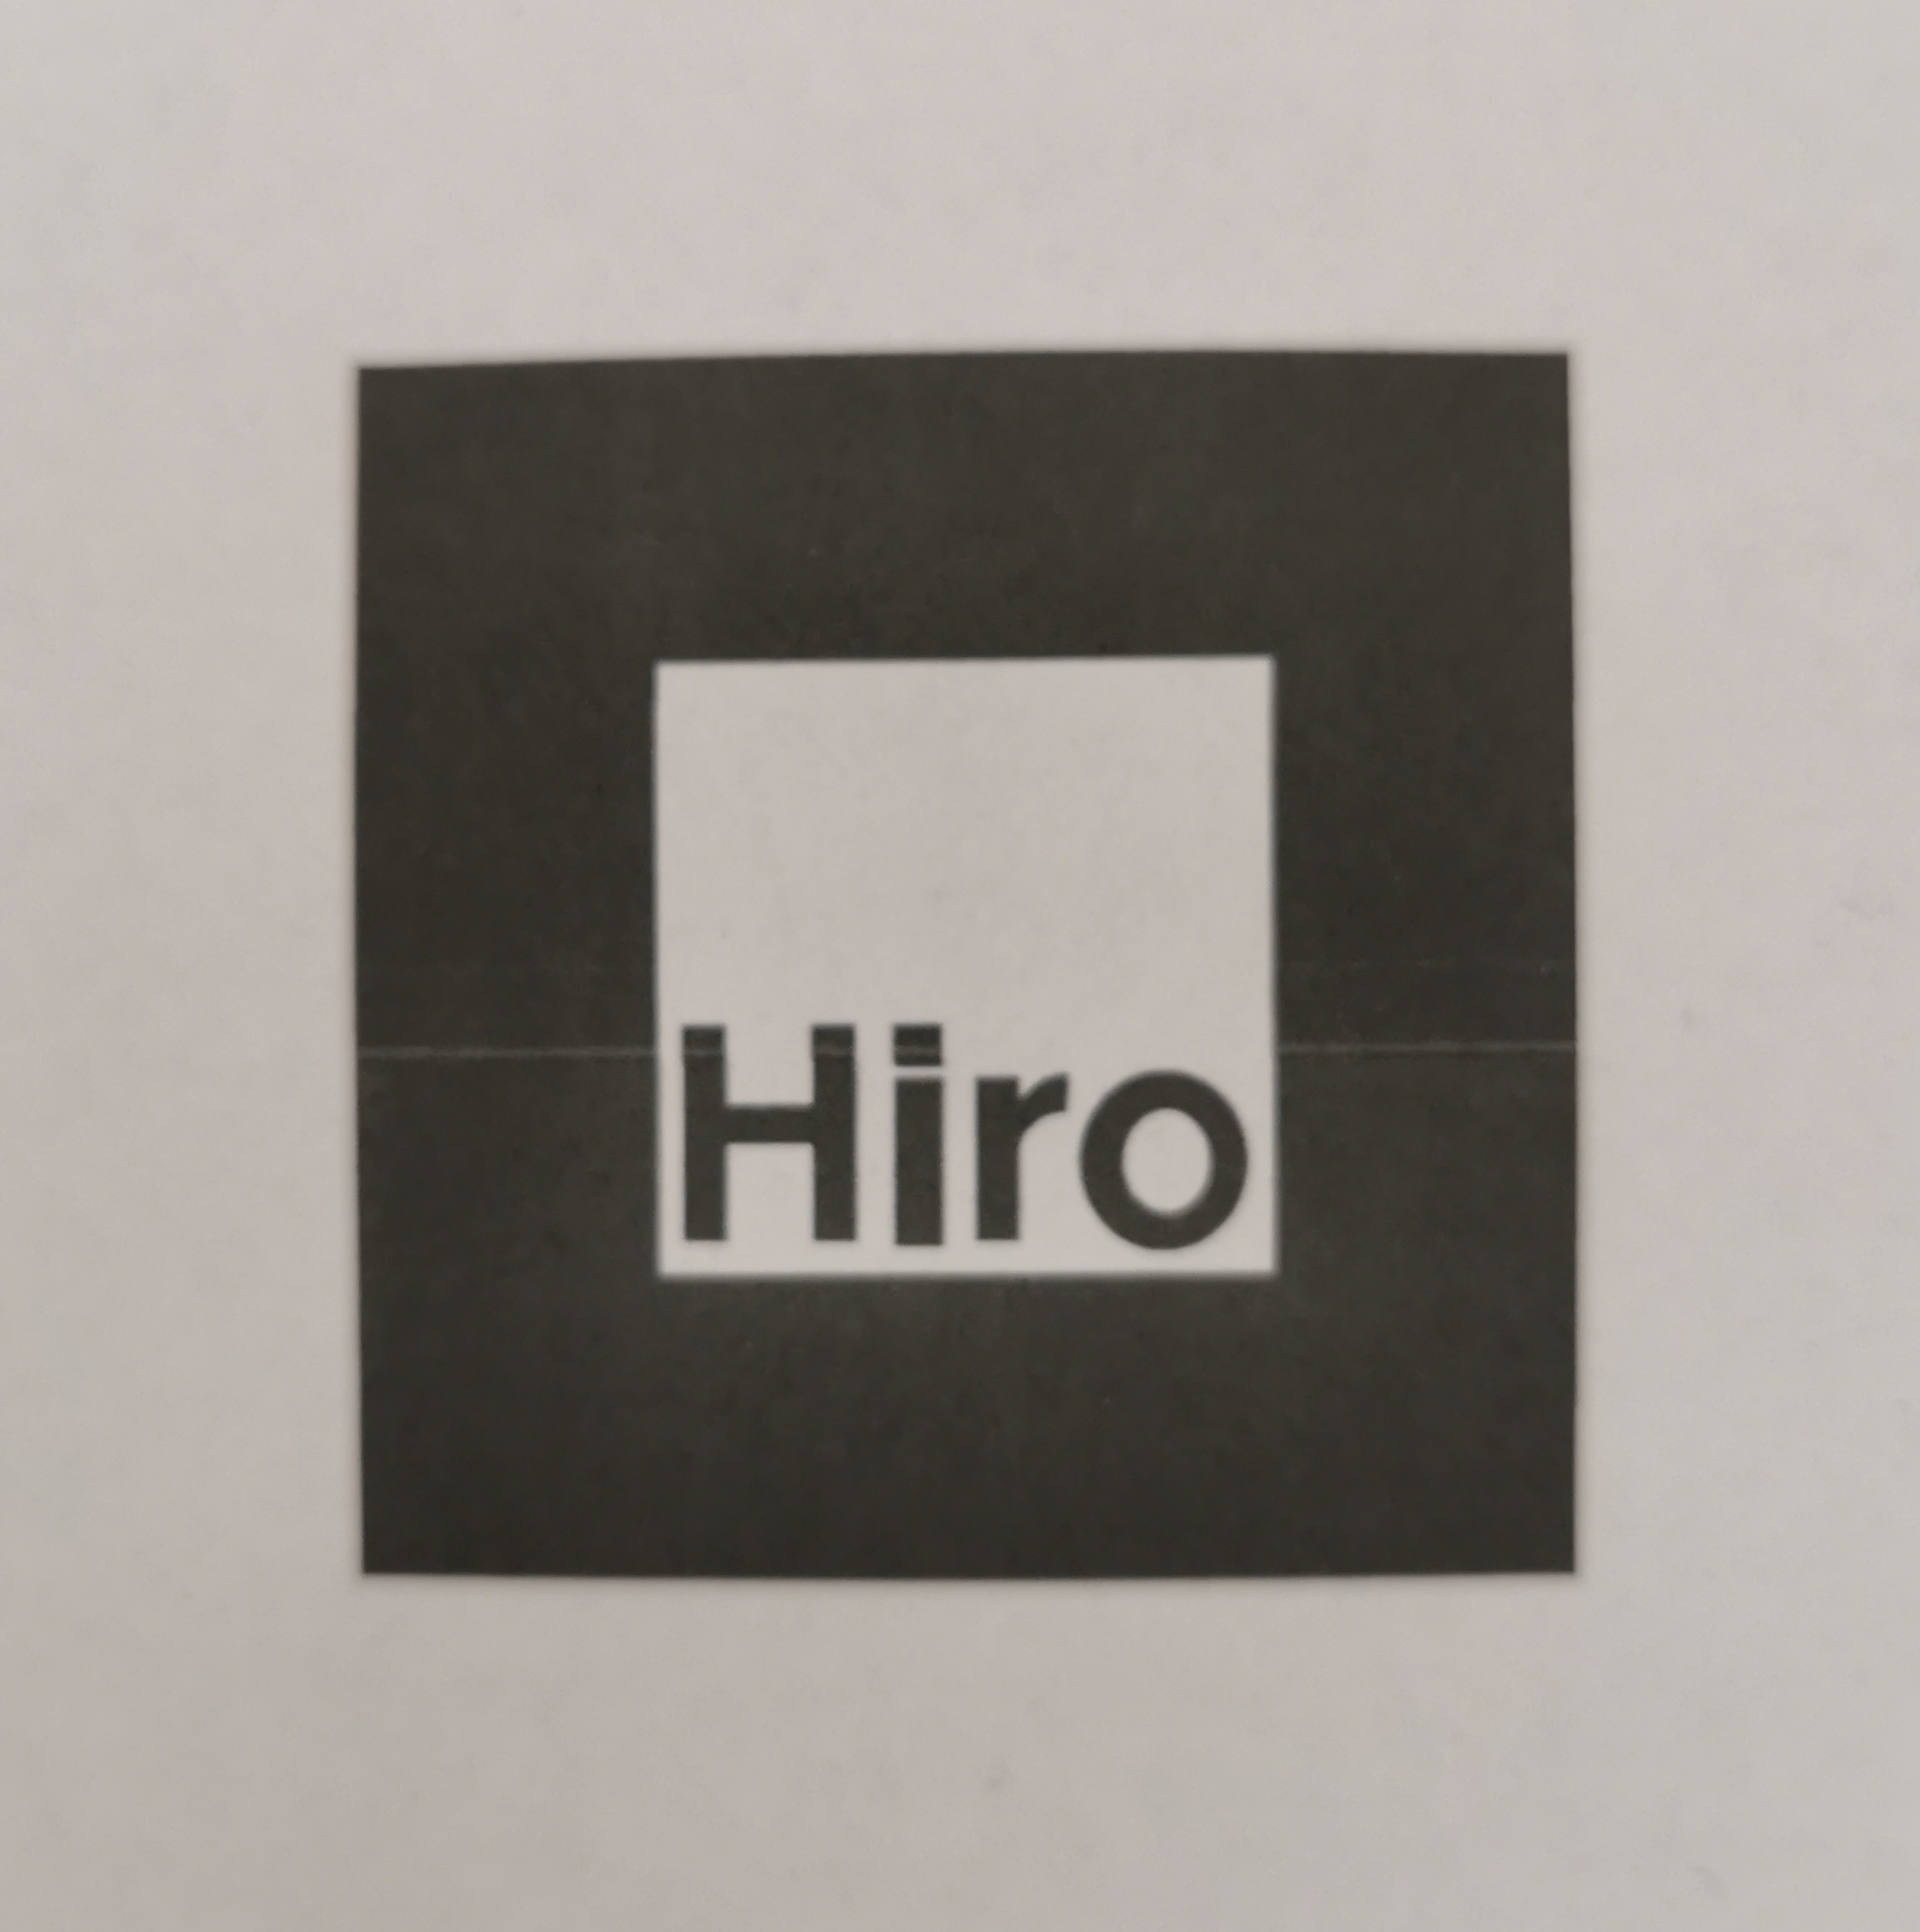
\includegraphics[width=0.2\textwidth]{Abbildungen/Invarianz/Skalierung1.jpg}
    
\includegraphics[width=0.2\textwidth]{Abbildungen/Invarianz/Skalierung2.jpg}
    \caption[Skalierungen eines Markers]{Verschiedene Skalierungen eines Markers. (Quelle: Eigene Darstellung)}
\end{figure}

\item Rotationsinvarianz: Dieser Testfall diente dazu das Tracking von Markern mit unterschiedlichen Rotationen zu testen, dazu wurde die Kamera auf das Dokument gerichtet und anschließend wurde letzteres langsam rotiert, um zu evaluieren, ob die Marker auch mit unterschiedlichen Rotationen korrekt erkannt werden.
\begin{figure}[H]
    \centering
    
\includegraphics[width=0.2\textwidth]{Abbildungen/Invarianz/Rotation1.jpg}
    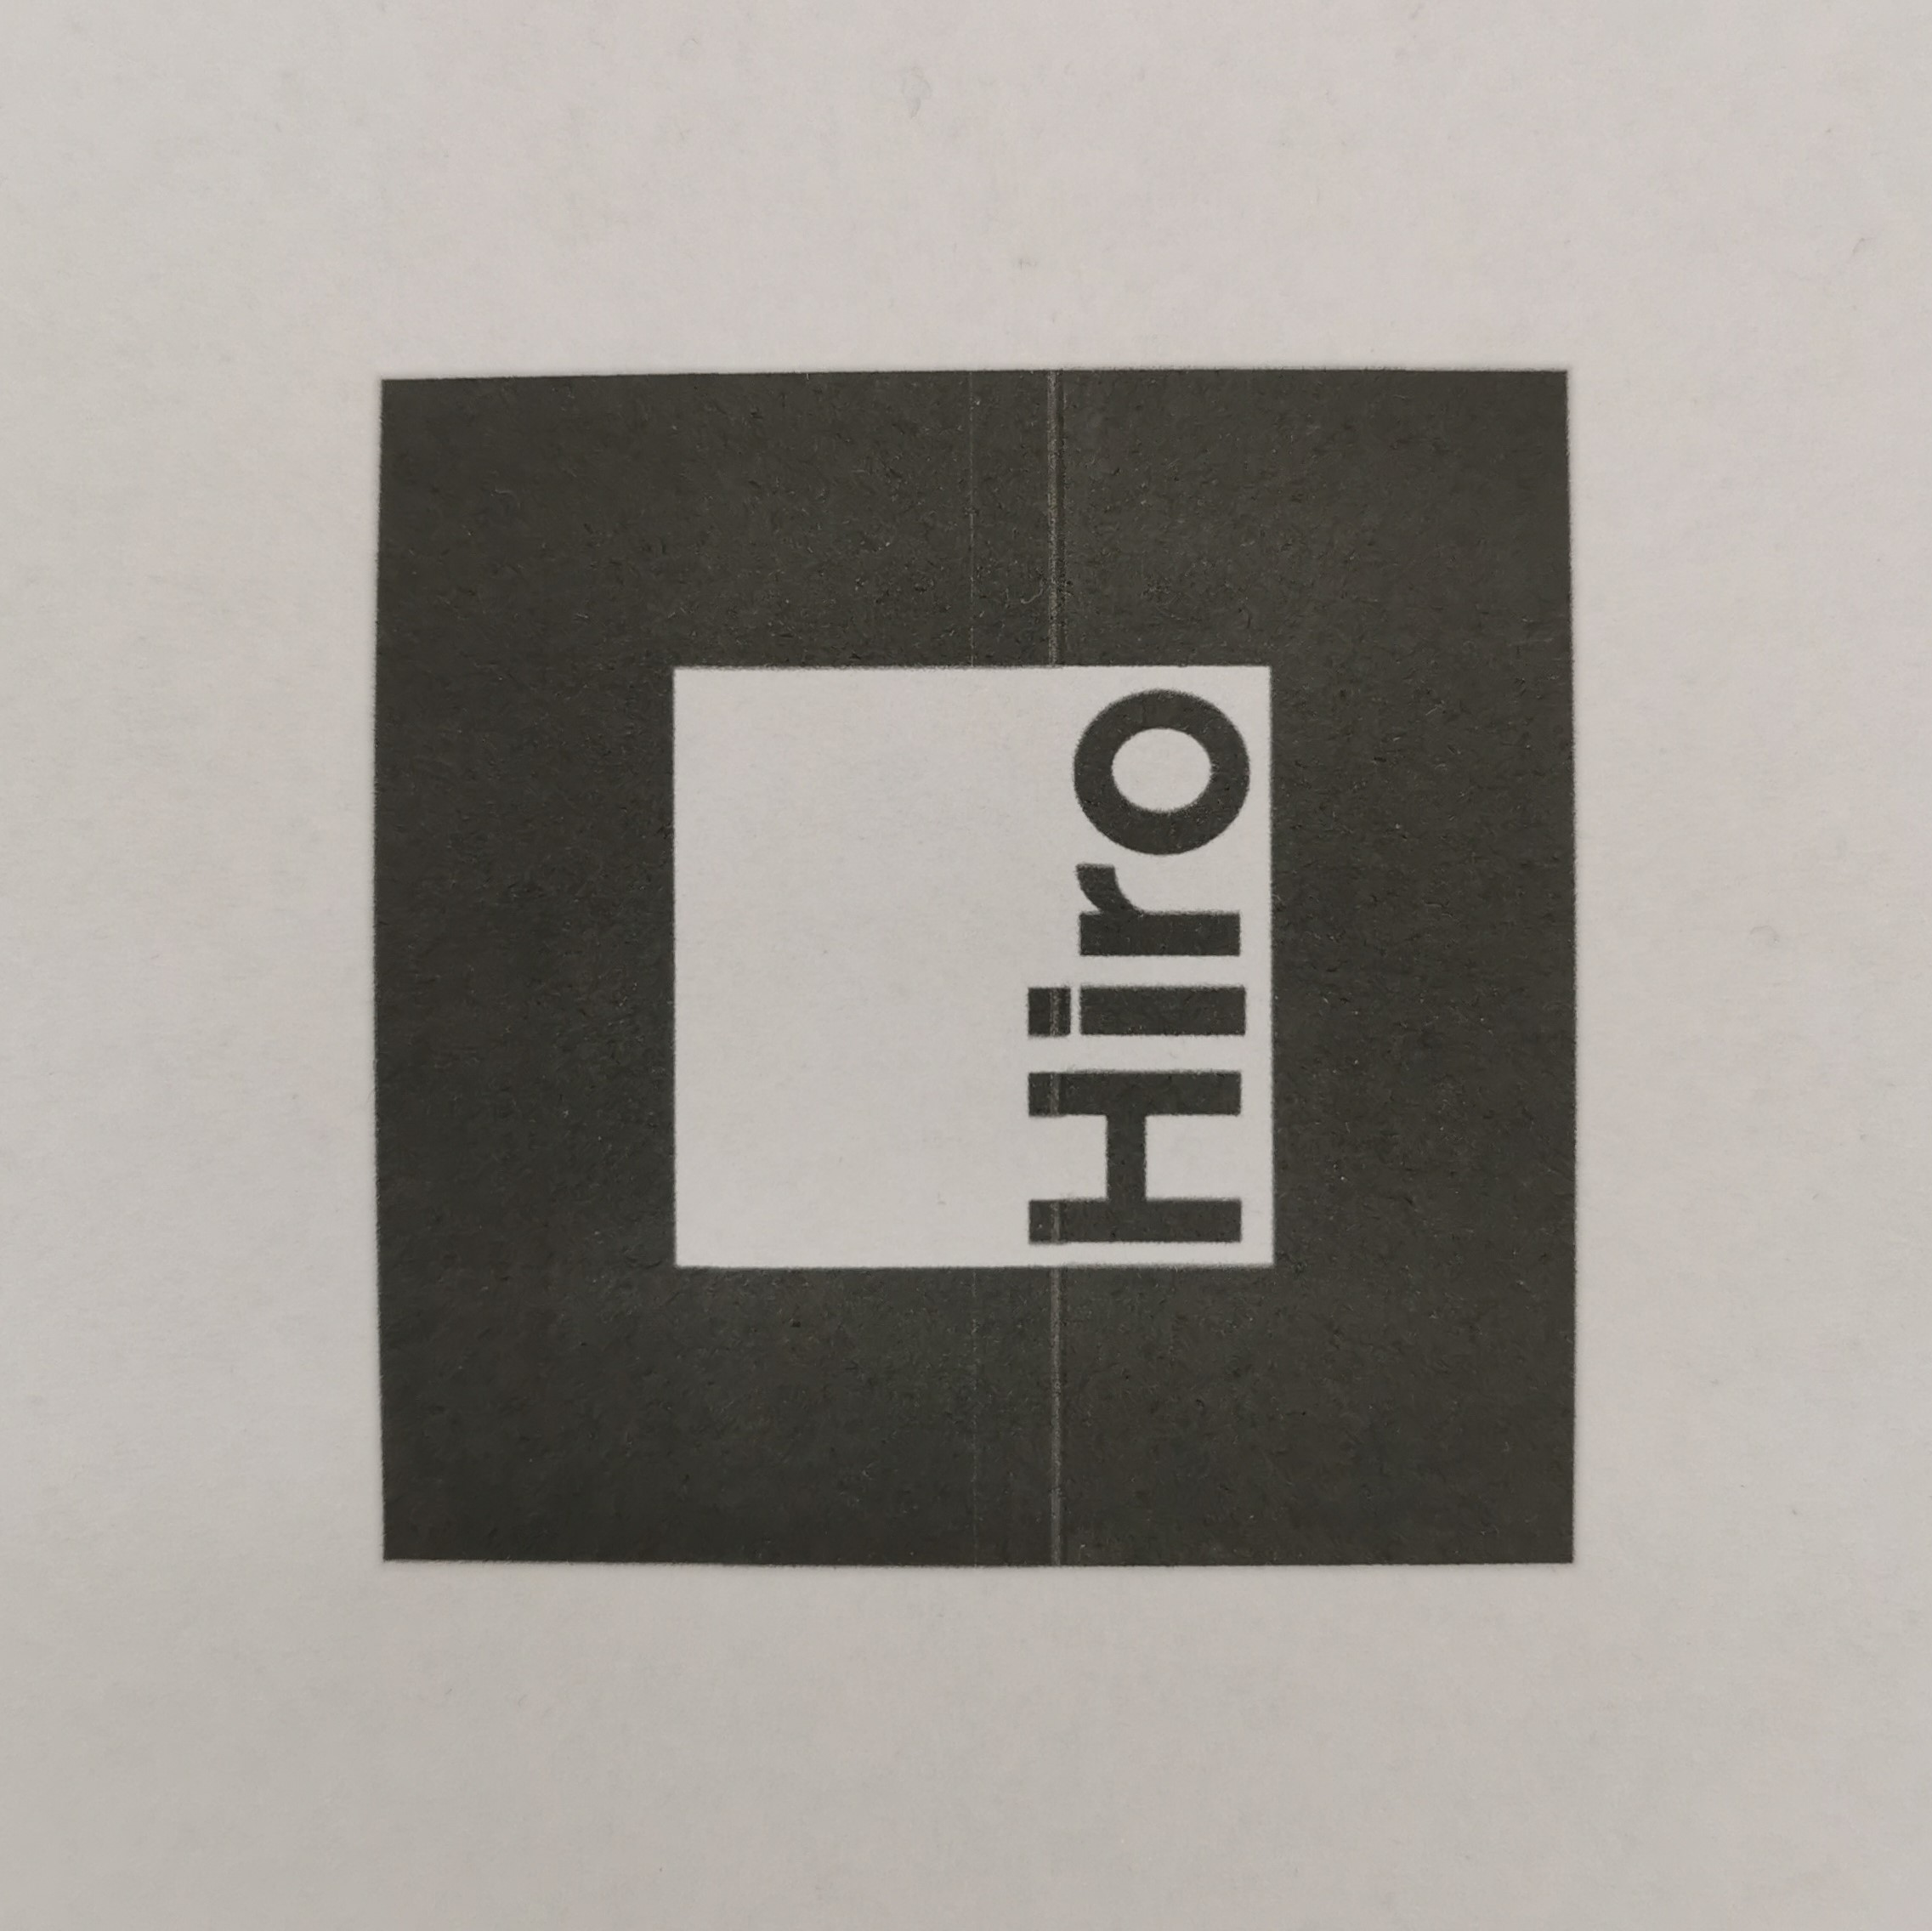
\includegraphics[width=0.2\textwidth]{Abbildungen/Invarianz/Rotation2.jpg}
    \caption[Rotationen eines Markers]{Verschiedene Rotationen eines Markers. (Quelle: Eigene Darstellung)}
\end{figure}

\item Belichtungsinvarianz: Dieser Testfall diente dazu das Tracking von Markern gegenüber unterschiedlichen Belichtungen zu testen. Dazu wurde mit Hilfe einer Lampe die Belichtung des Testdokumentes verändert.
\begin{figure}[H]
  	\centering
    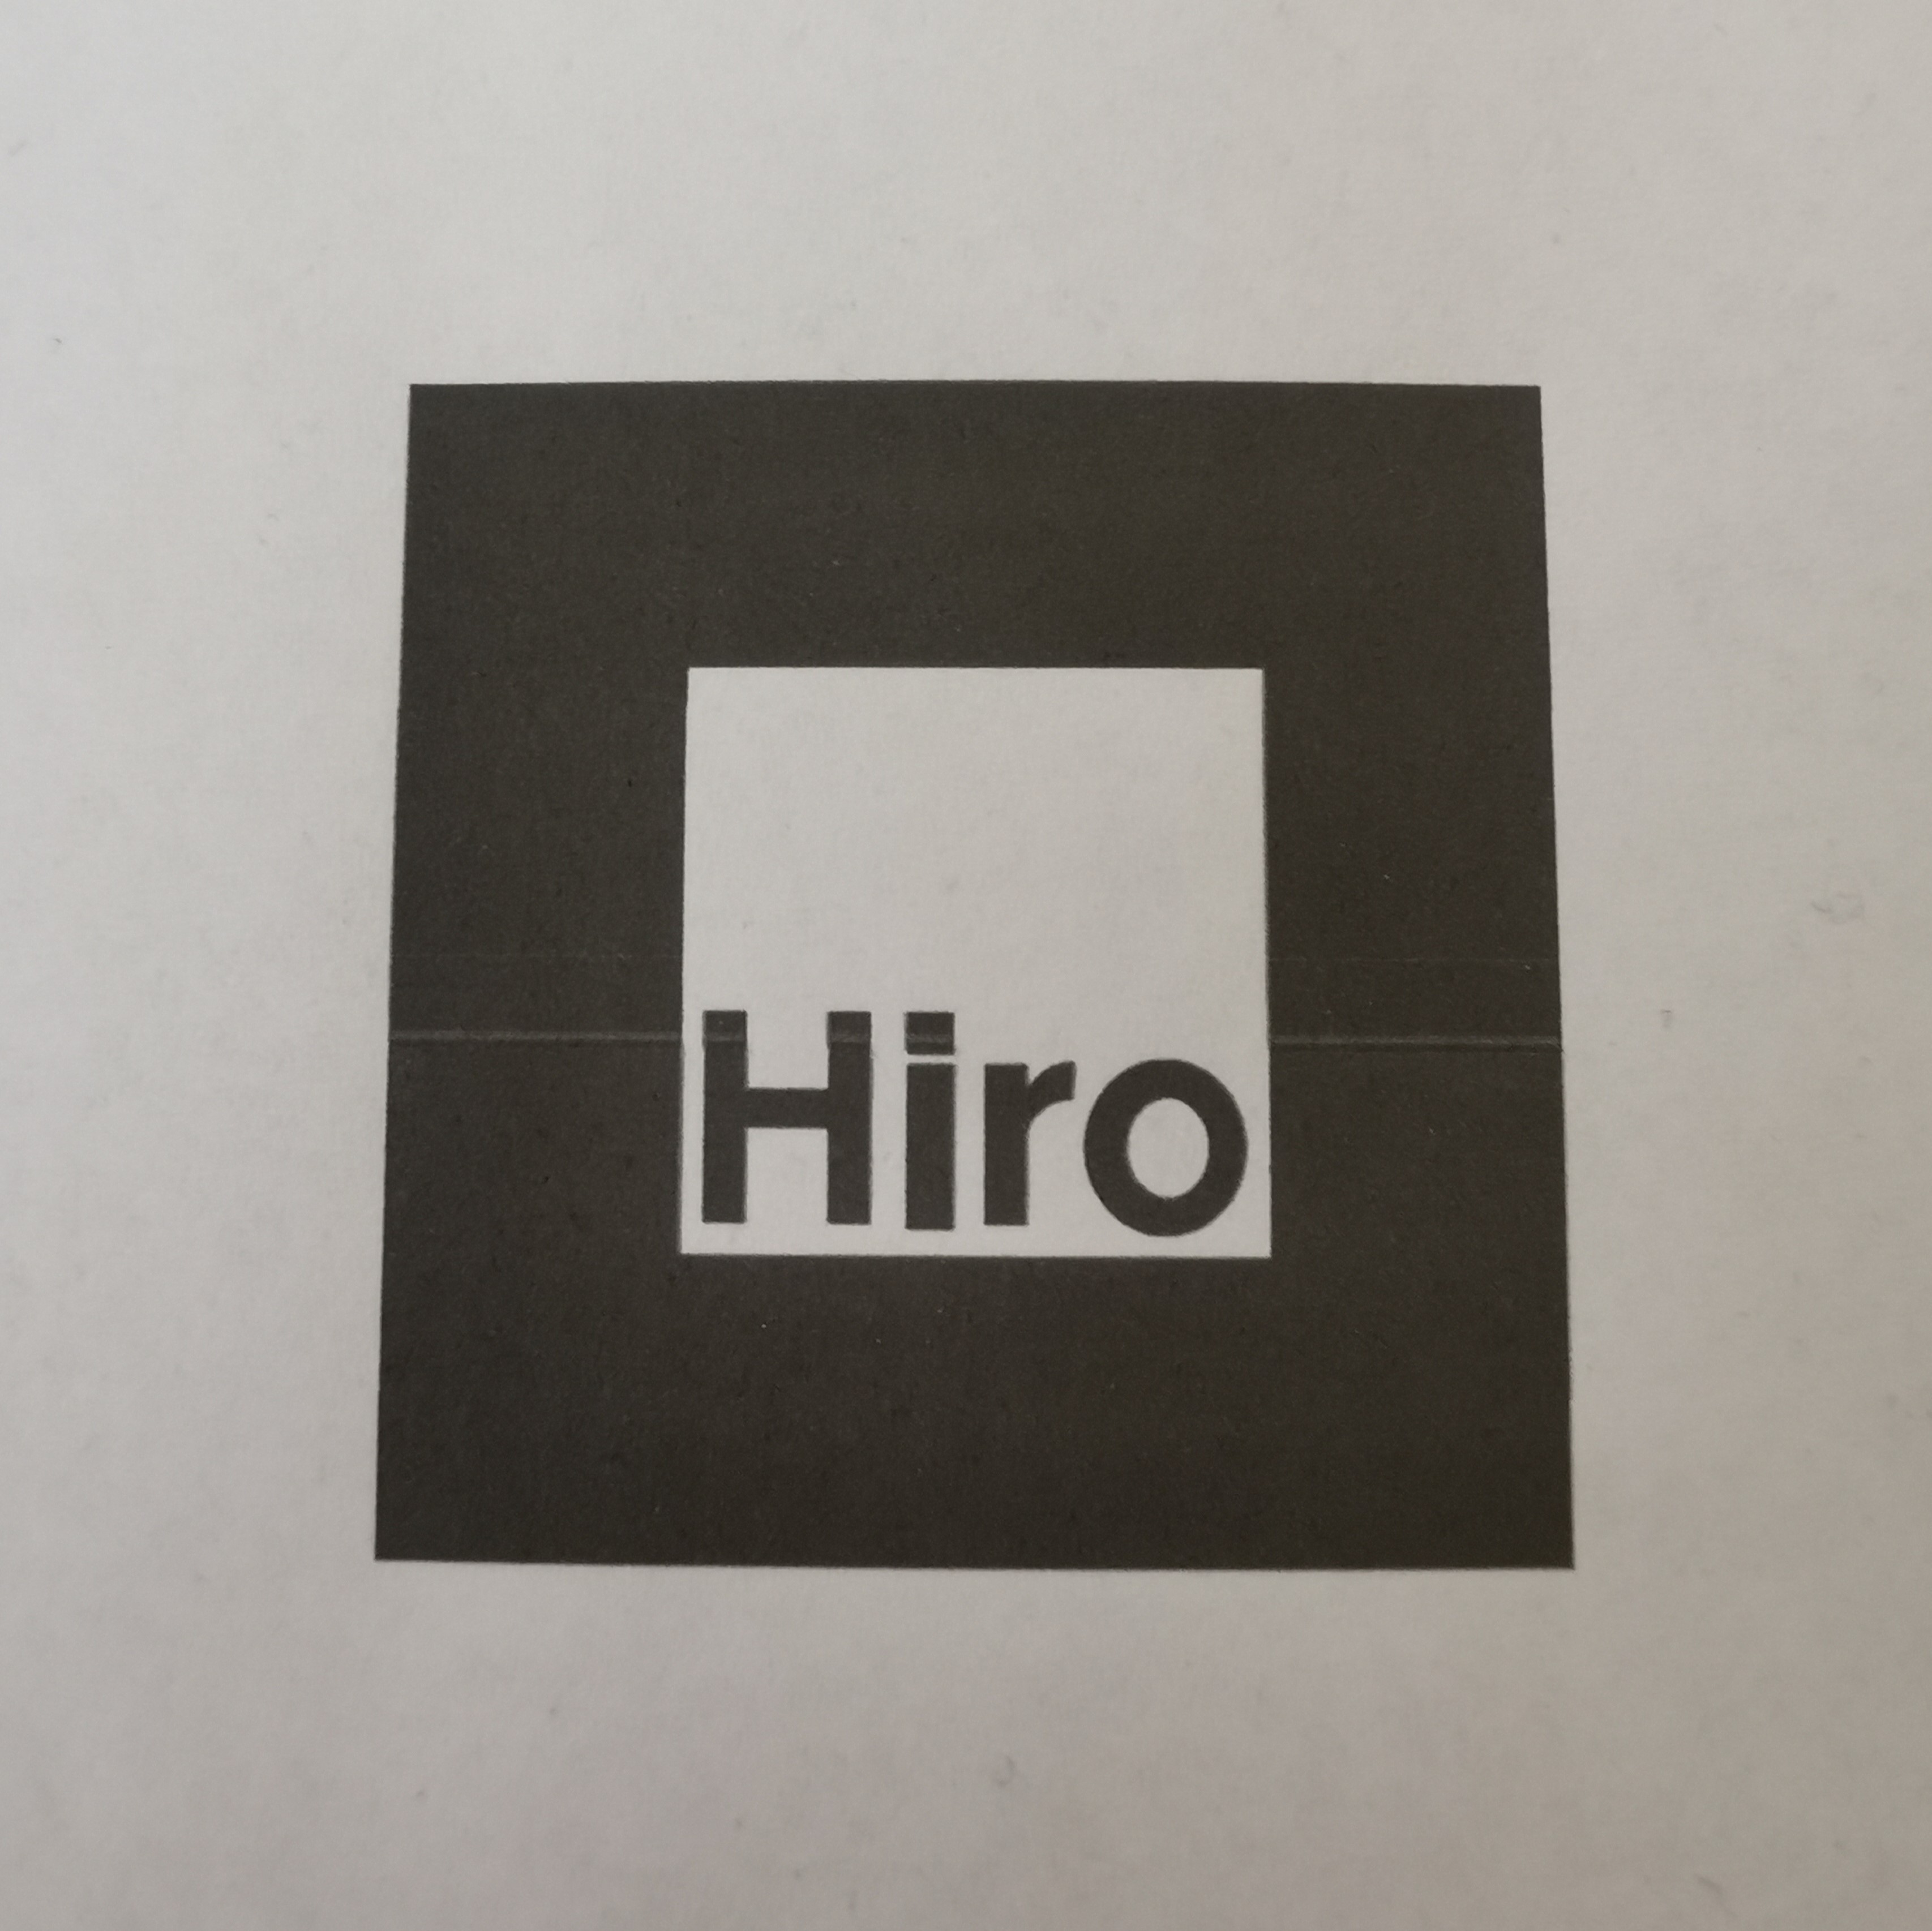
\includegraphics[width=0.2\textwidth]{Abbildungen/Invarianz/Belichtung1.jpg}
    
\includegraphics[width=0.2\textwidth]{Abbildungen/Invarianz/Belichtung2.jpg}
    \caption[Belichtungen eines Markers]{Verschiedene Belichtungen eines Markers. (Quelle: Eigene Darstellung)}
\end{figure}

\item  Trackinggeschwindigkeit:\todo{Besserer Name} Dieser Testfall sollte die Geschwindigkeit des Trackings, sowie die Robustheit testen. Dazu wurden ein oder mehrere Marker kurzzeitig mit der Hand verdeckt, um zu testen,ob anschließend alle Marker wieder erfolgreich getrackt wurden und wie schnell dieses erfolgte.
\end{itemize}
All diese Testfälle beziehen sich auf das Marker Tracking, während dessen konnten jedoch auch das Rendern des Modells und weitere Features die nicht direkt mit dem Tracking zusammenhängen getestet werden.\\

\subsubsection{Markergenerierung}
Um die Markergenerierungsfunktion des Prototyps zu testen wurden über der Programmcode der Anwendung so angepasst, dass die Nummer des getrackten Markers in der Konsole ausgegeben wurde. Anschließend wurden mit Hilfe der Anwendung eine Stcihprobe von fünf Markern generiert. Für die Stichprobe wurden dabei sowohl die äußeren Grenzen 0 und 4194303, als auch drei zufällig generierte Werte zwischen den beiden Grenzen gewählt.\\
Nun wurden zuletzt die generierten Marker manuell in das Tracking eingefügt und die Ausgabe mit der ID verglichen.

\subsubsection{Laden eigener Modelle}
Das Laden und verwenden eigener Modell-Dateien wurde getestet in dem eine Reihe an eigenen Modellen hochgeladen wurde und anschließend mit der Anwendung getrackt wurde.

\subsection{Bewertung des finalen Prototyps}




\subsection{Zusammenfassung}\label{sec:Zusammenfassung}
\todo{Am Ende schreiben}
- Belichtung nicht einfach zu testen
- starke Belichtungswechsel teilweise kurze Aussetzer

